\section{Introduction}  

We study a fundamental geometric invariant of compact sets, called the \textit{lattice diameter}, with a variety of applications in discrete geometry, integer optimization, and the geometry of numbers. We are not the first to study lattice diameters.
This notion was introduced by Corzatt and \mbox{Stolarsky~\cite{Corzatt_PhD}, 
% who were interested in minimal covers of lattice polygons, i.e., the smallest number of lines that cover all lattice points in the polygon. 
%Corzatt's conjecture, which is still open, states that any lattice polygon has a minimal cover using lines in at most four different directions.
studied} by Alarcon~\cite{Alarcon_PhD} and later by Bárány and Füredi~\cite{Barany_Furedi}. Here are the key definitions of this paper: 

\begin{definition}\label{def:ld-non-convex}
    For a compact set $S \subset \R^d$, define $$\ldiam(S):=\max_{\bx,\by \in S \cap \Z^d} |\conv(\{\bx,\by\}) \cap \Z^d|-1$$
    as the \emph{lattice diameter} of $S$. If $\bx$ and $\by$ maximize $\ldiam(S)$, we call $\conv(\{\bx,\by\})$ a \emph{lattice diameter segment}. Similarly, $\aff(\{\bx,\by\})$ is a \emph{lattice diameter line}, and finally, $\by-\bx$ or any of its non-zero multiples is called a \emph{lattice diameter direction}. 
\end{definition}

Our paper investigates properties of lattice diameter segments and algorithms to compute them.

Note that the lattice diameter of $S$ and $\conv(S)$ can differ when $S$ is non-convex. When $S$ is a convex body, then a lattice diameter line is an affine lattice line $L$ such that $|L \cap S \cap \Z^d|$ is maximal among all affine lattice lines. In this case the lattice diameter of $S$ coincides with the lattice diameter of $\conv(\{S \cap \Z^d\})$, a lattice polytope, thus we focus on studying lattice diameters of lattice polytopes. The Euclidean diameters and lattice diameters of lattice polytopes need not correlate. For fixed lattice diameter, the Euclidean diameter can be arbitrarily large (\Cref{fig:unbounded_ed}). Moreover, Euclidean diameter lines always pass through vertices \cite[Lemma~1.7]{GritzmannKlee1992}, while lattice diameter lines \mbox{may not (\Cref{fig:LL_interior}).}
\begin{figure}[ht!]
  \centering

  \begin{subfigure}[t]{0.48\textwidth}
    \centering
    \begin{tikzpicture}[thick, scale=0.9, baseline=(current bounding box.north)]
      % unify bbox across BOTH subfigures
      \path[use as bounding box] (0,0) rectangle (7,5);

      \foreach \x in {0,...,7} {
        \foreach \y in {2,...,4} {
          \node at (\x,\y) [circle, draw=lightgray, fill=lightgray, minimum width=2pt] {};
        }
      }

      \draw[line width=0.3mm] (0,2) -- (5,3) -- (7,4) -- (2,3) -- cycle;
      \draw[line width=0.4mm, lightgreen] (0,2) -- (7,4);
      \draw[line width=0.3mm, orange]     (2,3) -- (5,3);

      \foreach \x in {2,...,5} \node at (\x,3) [circle, fill=orange, minimum width=4pt] {};

      \node at (1.1,3) [black]{$(0,0)$};
      \node at (5.9,3) [black]{$(\ell,0)$};
      \node at (0.5,1.6) [black]{$(-n,-1)$};
      \node at (6.5,4.4) [black]{$(\ell+n,1)$};
    \end{tikzpicture}
    \caption{Lattice polygons with fixed lattice diameter \mbox{(orange)} and \mbox{unbounded} Euclidean diameter (green).}
    \label{fig:unbounded_ed}
  \end{subfigure}\hfill
  \begin{subfigure}[t]{0.48\textwidth}
    \centering
    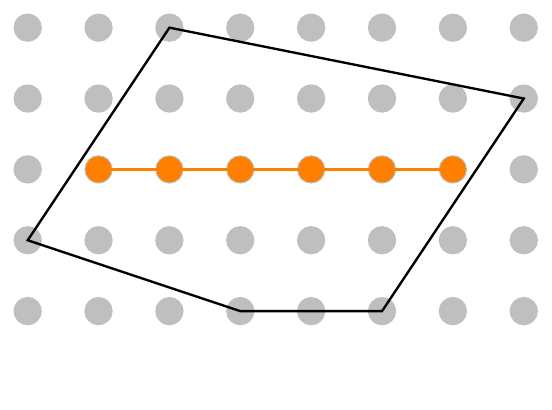
\begin{tikzpicture}[thick, scale=0.9, baseline=(current bounding box.north)]
      % unify bbox across BOTH subfigures
      \path[use as bounding box] (0,0) rectangle (7,5);

      \foreach \x in {0,...,7} {
        \foreach \y in {1,...,5} {
          \node at (\x,\y) [circle, draw=lightgray, fill=lightgray, minimum width=2pt] {};
        }
      }
      \draw[line width=0.3mm] (5,1) -- (7,4) -- (2,5) -- (0,2) -- (3,1) -- cycle;
      \draw[line width=0.3mm, orange] (1,3) -- (6,3);
      \foreach \x in {1,...,6} \node at (\x,3) [circle, fill=orange, minimum width=4pt] {};
    \end{tikzpicture}
    \caption{A lattice diameter segment contained in the interior of a lattice polygon.}
    \label{fig:LL_interior}
  \end{subfigure}

  \caption{Examples of lattice diameter segments in lattice polygons.}
  \label{fig:two_subfigs}
\end{figure}


% \begin{figure}[ht!]
%     \centering
%     % Left figure
%     \begin{minipage}[b]{0.48\textwidth}
%         \centering
%         \begin{tikzpicture}[thick, scale=0.9, baseline=(current bounding box.south)]
%             % unify bbox across BOTH figures
%             \path[use as bounding box] (-0.5,0.5) rectangle (7.5,5.5);

%             \foreach \x in {0,...,7} {
%                 \foreach \y in {2,...,4} {
%                     \node at (\x,\y) [circle, draw=lightgray, fill= lightgray, minimum width=2pt] {};   
%                 }
%             }

%             \draw[line width=0.3mm, black] (0,2) -- (5,3) -- (7,4) -- (2,3) -- cycle;
%             \draw[line width=0.4mm, lightgreen](0,2) -- (7,4);
%             \draw[line width=0.3mm, orange](2,3) -- (5,3);
            

%             \foreach \x in {2,...,5} {
%                 \node at (\x,3) [circle, fill=orange, minimum width=4pt] {};
%             }

%             % \node at (0,2) [circle, fill=black, minimum width=4pt] {};
%             % \node at (7,4) [circle, fill=black, minimum width=4pt] {};

%             \draw(1.1,3) node[black]{$(0,0)$};
%             \draw(5.9,3) node[black]{$(\ell,0)$};
%             \draw(0.5,1.6) node[black]{$(-n,-1)$};
%             \draw(6.5,4.4) node[black]{$(\ell+n,1)$};
%         \end{tikzpicture}
%         \caption{A lattice polygon with fixed \mbox{lattice} diameter (orange) and arbitrarily long \mbox{Euclidean} diameter (green).}
%         \label{fig:unbounded_ed}
%     \end{minipage}
%     \hfill
%     % Right figure
%     \begin{minipage}[b]{0.48\textwidth}
%         \centering
%         \begin{tikzpicture}[thick, scale=0.9, baseline=(current bounding box.south)]
%             % unify bbox across BOTH figures
%             \path[use as bounding box] (-0.5,0.5) rectangle (7.5,5.5);

%             \foreach \x in {0,...,7} {
%                 \foreach \y in {1,...,5} {
%                     \node at (\x,\y) [circle, draw=lightgray, fill= lightgray, minimum width=2pt] {};   
%                 }
%             }
%             \draw[line width=0.3mm, black] (5,1) -- (7,4) -- (2,5) -- (0,2) -- (3,1) -- cycle;

%             % segment
%             \draw[line width=0.3mm, orange](1,3) -- (6,3);

%             \foreach \x in {1,...,6} {
%                 \node at (\x,3) [circle, fill=orange, minimum width=4pt] {};
%             }
%         \end{tikzpicture}
%         \caption{A lattice diameter segment \mbox{in the interior} of a lattice polygon.}
%         \label{fig:LL_interior}
%     \end{minipage}
% \end{figure}
% % \begin{figure}[ht!]
% %     \centering
% %         \begin{tikzpicture}[thick, scale=1]\vspace{0.5cm}
% %         \draw[line width=0.3mm, white](-3,-1.5) -- (6,-1.5);
    
% %         \foreach \x in {-2,...,5} {
%             \foreach \y in {-1,...,1} {
%                 \node at (\x,\y) [circle, draw=lightgray, fill= lightgray, minimum width=1pt] {};   
%             }
%         }
    
%          \draw[line width=0.3mm, black] (-2,-1) -- (3,0) -- (5,1) -- (0,0)-- cycle;
%          \draw[line width=0.3mm, orange](0,0) -- (3,0);
%          \draw[line width=0.3mm, lightgreen](-1.9,-1) -- (4.9,1);

%          \foreach \x in {0,...,3} {
%                 \node at (\x,0) [circle, fill=orange, minimum width=4pt] {};
%             }
%         \node at (-2,-1) [circle, fill=black, minimum width=4pt] {};
%         \node at (5,1) [circle, fill=black, minimum width=4pt] {};

%         \draw(-0.8,0.3)node[black]{$(0,0)$};
%         \draw(4.1,-0.3)node[black]{$(\ell-1,0)$};
%         \draw(-1.6,-1.5)node[black]{$(-n,-1)$};
%         \draw(4.8,1.3)node[black]{$(\ell-1+n,1)$};
        

%     \end{tikzpicture} \vspace{-0.5cm}
    
%     \caption{unbounded Euclidean diameter for fixed lattice diameter}
%     \label{fig:unbounded_ed}
% \end{figure}
% \begin{figure}[ht!]
%     \centering
%     \includegraphics[width=0.8\linewidth]{Figures/1.0_unbounded-ed.png}
%     \caption{unbounded Euclidean diameter for fixed lattice diameter}
%     \label{fig:unbounded_ed}
% \end{figure}

Lattice lines and lattice diameter lines have several interesting connections. For example, in discrete tomography Gardner and Gritzmann have studied the reconstruction of lattice point sets from ``$X$-rays'', i.e., the collection of line sums over parallel lattice lines~\cite{gardnergritzmann97}. Algorithmic connections to combinatorial optimization also exist through the notion of \emph{lattice width}, which is used in algorithms for integer programming. The lattice width has been shown to be bounded by the lattice diameter \cite{Barany_Furedi}. Motivated by questions in the geometry of numbers, the volumes of sections and projections of convex bodies have been studied for many years; see the surveys \cite{giannopoulos2023inequalities, nayar2023extremal}. Analogous questions for the number of lattice points have only been studied more recently \cite{gard05,freyerhenk22,freyerhenk24}. Algorithmically, it is a challenge to determine a section of a convex body with maximal volume, but algorithms exist for convex polytopes~\cite{BDLM}. However, computing a section of a lattice polytope with the most lattice points is still an open problem. In the plane, this problem reduces to finding a lattice diameter segment, which we solve here. 

%Classical inequalities – such as those of Loomis–Whitney~\cite{} and Bourgain’s slicing problem~\cite{} — seek optimal bounds relating the volume of a convex body to the volume of its sections or, dually, 

Furthermore, classifications of convex lattice polytopes have been studied with respect to different invariants. This is of particular interest in algebraic geometry, where reflexive polytopes correspond to specific toric Fano varieties that have ties to mirror symmetry in physics~\cite{batyrev1999classification, kasprzyk2006toric}. Arnold, B\'ar\'any, Pach, Vershik, and others~\cite{arno80, bara92, bara92a} have classified lattice polytopes by their volume while Averkov, Lagarias, Nill, Weismantel, Ziegler, and others \cite{lagariasZiegler1991bounds, averkov2011maximal, nillziegler2011projecting} have continued the classification, based on the number of interior lattice points. We stress that classifying lattice polytopes by their lattice diameter is also possible. A simple result by S. Rabinowitz \cite{rabi89} shows that if $\ldiam(P)<m$, then $|P \cap \Z^d| \leq m^d$.
%, for a lattice polytope $P$.
% \begin{proposition}[\cite{rabi89}]\label{lemma:Rabinowitz}
% Let $P$ be a $d$-dimensional convex lattice polytope and let $m \in \N$ satisfy $|P \cap \Z^d|\geq m^d+1$. Then $P$ has at least $m+1$ collinear lattice points. In other words, if  $\ldiam(P) < m$, then $|P \cap \Z^d| < m^d+1$.
% \end{proposition}
Also in more recent work, Dillon and Arun~\cite{HollowP} asymptotically bound the number of vertices that a lattice polytope with fixed lattice \mbox{diameter can have.}


%For $n=2$ the proof is an elementary pigeon-hole argument. If $|P \cap \Z^d| \geq 2^d$, then there would exist $x,y \in P \cap \Z^d$ whose coordinates all have the same parity, thus the midpoint $\frac{1}{2}x+\frac{1}{2}y \in P \cap \Z^d$ yielding three collinear points in $P$.

% \begin{proof}Consider the coordinates of the integer points modulo $m$.
% Since there are only $m^d$ distinct $d$-tuples of integers modulo
% $m$, some two points ${\bf x}$ and ${\bf y}$ of $P\cap \mathbb{Z}^d$ must be
% congruent (mod $m$). In other words, for all $i=1, 2, \ldots , d$, we have
% $$x_i-y_i\equiv 0\quad ({\rm mod}\ m).$$
% By convexity, all the $m+1$ collinear lattice points
% $${\bf x}+\mbox{${j\over m}$}({\bf y}-{\bf x}),\quad j=0, 1, 2, \ldots
% , m$$ belong to $P$. The lemma is proved.
% \end{proof}

% Furthermore, in the plane Pick's Theorem~\cite{pick99} turns Rabinowitz's bound into an upper bound on the area of $P$ in terms of its lattice diameter. 

Another theme of our paper is Ehrhart theory. In its simplest version, for a $d$-dimensional lattice polytope $P$, and $k \in \N$, the Ehrhart counting function, $\Ehr_P(k) = |kP \cap \Z^d|$, agrees with a polynomial in $k$ of degree $d$. This foundational result extends to rational, multivariate, and weighted versions, using generating functions and featuring reciprocity theorems \cite{beckrobins}. Here we count not individual lattice points, but subsets of them.
It can be shown that there is an Ehrhart theorem for counting lattice lines with fixed direction in a rational polytope, that pass through a lattice point of the rational polytope \cite{aebThesis}.
% It was observed by the second author and collaborators that one has a similar Ehrhart theorem for counting lattice lines in a fixed direction $\bu \in \Z^d$ that contain a lattice point of a rational polytope \cite{unifiedEtheory}. 
In this paper we study the counting function of lattice diameter lines (or segments) of a lattice polygon.

A final motivation for our work is the famous Borsuk's partition problem. In 1933, Borsuk posed the following question in \cite{borsuk1933drei}:
\begin{quote}
    \emph{Can every bounded set $S \subset \R^d$ be partitioned into $d+1$ sets with \mbox{smaller diameter?}}
\end{quote}
Here \textit{diameter} refers to the Euclidean diameter, i.e., $\diam(S) := \max_{\bx,\by \in S} \|\bx-\by\|_2$ where $\| \cdot \|_2$ is the Euclidean norm.
The answer to Borsuk's question is positive for $d=2$, see \cite{borsuk1933drei}, and for $d=3$, see \cite{perkal1947subdivision}, \cite{eggleston1955covering} and \cite{grunbaum1957simple}. In higher dimensions it was believed to be true until Kahn and Kalai \cite{kahn1993counterexample} constructed a counterexample for $d=1325$ and for each $d>2014$. Today, there are known counterexamples in dimensions $64$ and higher, see \cite{jenrich201464}, but the problem is still open for $4\leq d\leq 63$.
More generally, the problem of partitioning a set into sets with smaller diameter is studied for specific classes of bounded sets. In this paper, we study this problem for sets of lattice points with respect to the lattice diameter instead of the Euclidean diameter. We refer to this challenge as the \textit{discrete Borsuk partition problem}.

\subsection*{Our Contributions}

In \Cref{sec:LD-poly} we show that lattice diameter lines of lattice polygons can be computed efficiently:

\begin{manualthm}\emph{\textbf{Theorem~2.4.}}
    Let $P \subset \R^2 $ be a lattice polygon. There exists a polynomial-time algorithm that computes a lattice diameter line of $P$ in every direction in which such a line exists. In particular, the lattice diameter of $P$ can be computed in polynomial time.
\end{manualthm} 

In contrast, we show the following hardness result in \Cref{sec:NP-hard}:

\begin{manualthm}\textbf{\emph{Theorem~2.7.}}
    Let $d \geq 3$ and let $K \subset \R^d$ be a $d$-dimensional bounded semi-algebraic set. \mbox{Computing} a lattice diameter of $K$ is an $\NP$-hard problem. 
    %Moreover, even computing a $\bu$-lattice diameter of $K$ in a fixed direction $\bu \in \Z^d \setminus \{0\}$ is $NP$-hard.
\end{manualthm}

In \Cref{sec:QP} we generalize Ehrhart theory to counting the set of lattice diameter lines. While counting the number of lattice lines in a fixed direction that intersect $P$ in a lattice point is not hard \cite{aebThesis}, counting those that are lattice diameter lines is much more difficult. Surprisingly, we have an Ehrhart-type result.

\begin{definition}\label{def:LD_P}
    For a lattice polytope $P$, let $\LD_P(k)$ denote the number of lattice diameter lines of the dilated polytope $kP$.
\end{definition}

\begin{manualthm}
    \emph{\textbf{Theorem~3.6.}} Let $P \subset \R^2$ be a lattice polygon. There exists a positive integer $q$ such that \mbox{$\LD_P: \N_{\geq q} \to \N$} agrees with a quasi-polynomial function of degree one whose period divides $q$.
\end{manualthm}

 In \Cref{sec:directions-Borsuk} we begin by generalizing two results by Alarcon~\cite{Alarcon_PhD} to higher dimensions. The first result bounds the total number of lattice diameter directions:

\begin{manualthm}\textbf{\emph{Theorem~4.3.}}
    Let $P\subset \R^d$ be a lattice $d$-polytope with $\ldiam(P)=1$. Then $P$ has at most $\binom{2^d}{2}$ lattice diameter directions and this bound is best possible.
\end{manualthm}

The second generalization is about a local property of lattice diameter segments. In fact, we prove it more generally for bounded sets. This result is a key ingredient to prove the discrete version of Borsuk's partition problem.

\begin{manualthm}\textbf{\emph{Lemma~4.6.}}
    Let $S\subset \Z^d$ be a bounded set and let $\bx \in S$. Then, the number of lattice diameter segments of $S$ that have $\bx$ as an endpoint is bounded by $2^d-1$, and this bound is best possible.
\end{manualthm}

To study the discrete version of Borsuk's partition problem, we define the following notion:

\begin{definition}
    Let $S \subset \Z^d$ be a bounded set. Define the \textit{lattice Borsuk number} of $S$, $\beta_\Z(S)$, as the minimal size of a partition of $S$ where each part has a smaller lattice diameter than $\ldiam(S)$.
\end{definition}

Finally, the following theorem answers the discrete version of Borsuk's partition problem:

\begin{manualthm}\textbf{\emph{Theorem~4.8.}}
    Let $S \subset \Z^d$ be a bounded set. Then, $\beta_\Z(S) \leq 2^d$ and this bound is best possible.
\end{manualthm}

In particular, \Cref{Thm:Borsuk} says that $\beta_\Z(P \cap \Z^d) \leq 2^d$ for $d$-dimensional polytopes $P$. Note that we are not partitioning $P$ into smaller polytopes, i.e., the parts of $P \cap \Z^d$ are not necessarily the lattice points of a polytope. The bound $2^d$ is also best possible for polytopes; it is attained for the lattice points of a $d$-dimensional cube.

\subsection*{Notation}
We use basic notions and notation as can be found in the textbooks~\cite{grub07,zieglerbook}.
% A convex body means a compact convex set, and a lattice polytope in $\R^d$ is the convex hull of finitely many integer points in $\Z^d$.
%Vectors $\bv \in \R^d$ will be written bold.
A $d$-polytope $P$ is the convex hull of finitely many points in $\R^d$ whose affine hull is $d$-dimensional. It is called a \emph{lattice} (or \emph{rational}) $d$-polytope if its vertices belong to the integer lattice $\Z^d$ (or to $\Q^d)$. We say two lattice $d$-polytopes $P$ and $Q$ are unimodularly equivalent if there exists a unimodular matrix $A \in \GL(d,\Z)$ and $\bt \in \Z^d$ such that $P=AQ+\bt$, i.e., these transformations correspond to lattice preserving maps. We write $\spn(S), \, \aff(S)$, and $\conv(S)$ for the linear, affine, and convex hull of a set $S \subset \R^d$, respectively.
The segment between two points $\bx,\by \in \R^d$ is denoted $[\bx,\by]:=\conv(\{\bx,\by\})$ and when $\bx,\by \in \Z^d$, we call this a \textit{lattice segment}. A \emph{line} will always mean an \emph{affine line} and a \emph{lattice line} is a line that passes through at least two lattice points. We say that a line has direction $\bu$ if it can be written as $\bx+\spn(\bu)$ for some $\bx \in \R^d$. We say $\bu$-lattice line (or segment) if the lattice line (or segment) has direction $\bu$. Furthermore, from now on a \textit{diameter direction} means a lattice diameter direction. The inner product we use is the standard inner product on $\R^d$, denoted $\langle \cdot, \cdot \rangle$. A hyperplane and its closed half-spaces are denoted $H(\ba,\alpha):= \{ \bx \in \R^d \st \langle \ba, \bx \rangle = \alpha \}$, $H^+(\ba,\alpha)$ and $H^{-}(\ba,\alpha)$, respectively. For a Lebesgue measurable set $S\subset \R^d$, we write $\vol(S)$ which means the intrinsic volume of $S$ in $\aff(S)$. Furthermore, a vector $\bu=(u_1, \ldots, u_d) \in \Z^d$ is called primitive if $\gcd(u_1, \ldots, u_d) =1$. For a positive integer $n$ we write $[n]:=\{1, \ldots, n\}$ and $\binom{[n]}{k}$ denotes the $k$-element subsets of $[n]$. For integers $a,q \in \Z$ we write $a \bmod q$ to mean the representative of $a$ in $\{0, \ldots, q-1\}$.
%Lastly, the natural numbers $\N$ contain $0$.
%, and when we write $d \in \N$ for dimension we assume $d\geq 2$.
In \Cref{sec:directions-Borsuk}, we use graph theory and standard notation as in \cite{bondy2008graph}. A graph is a simple undirected graph $G=(V,E)$, where $V$ is a finite set and $E \subseteq \binom{V}{2}$. In this context, $V$ or $V(G)$ is the set of \emph{vertices} and $E$ or $E(G)$ is the set of \emph{edges} of the graph $G$. Two vertices $u,v\in V$ are called \emph{adjacent} if $\{u,v\} \in E$.

%OLD introduction notes

% \begin{definition}\label{def:ld-convex}
% Let $C \subset \R^d$ be a convex body. An affine lattice line $L$ is called a \textit{lattice diameter line} of $C$ if $|L \cap C \cap \Z^d| \geq | L' \cap C \cap \Z^d|$ for all affine lines $L'$. In this case $L \cap C$ is called a \emph{lattice diameter segment}, and $\ldiam(C):=|L \cap C \cap \Z^d|-1$ is called the \emph{lattice diameter} of $C$. Further, for a non-zero vector $\bu \in \Z^d$, a \textit{$\bu$-lattice line} $L$ is an affine lattice line $L$ with direction $\bu$. It is called a \textit{$\bu$-lattice diameter line} of $C$, if $L \cap C \cap \Z^d| \geq |L' \cap C \cap \Z^d|$ for all $\bu$-lattice lines $L'$ and in this case, $|L \cap C|$ is called a $\bu$-\emph{lattice diameter segment} and $|L \cap C \cap \Z^d|-1$ is called the $\bu$\textit{-lattice diameter} of $C$. If a $\bu$-lattice diameter line is a lattice diameter line of $C$, then $\bu$ is called a \textit{diameter direction} of $C$.
% \end{definition}

% counted the number of lattice polytopes with a fixed number of interior points and provide explicit upper bounds of the lattice diameter in terms of the dimension and the number of interior points. What happens when there are no lattice points in the interior? Lattice polytopes without interior points are of interest but their classification is incomplete. Nill and Ziegler~\cite{nillziegler2011projecting} showed that up to unimodular equivalence there are only finitely many $d$-dimensional lattice polytopes without interior lattice points that do not admit a lattice projection onto a ($d-1$)-dimensional lattice polytope without interior lattice points. This connects to work of  Averkov, Wagner and Weismantel~\cite{AverkovWW10}, on the finiteness of the number of maximal lattice polytopes without any interior lattice points. 

% Furthermore, convex lattice polytopes with bounded volume or few interior points have been classified in various settings~\cite{Arn80, BP92, BV92, LZ91, NZ11} [CHECK THESE CITATIONS!]. 